\documentclass[fleqn]{jbook}
\usepackage{physpub}

\begin{document}

\begin{question}{専攻 問題3}{}

\begin{subquestions}
\SubQuestion

\parbox[t]{110mm}{大きさ$\frac{1}{2}$のスピン2個が、次のハミルトニア
ンで相互作用している系を考える。
\[ {\cal{H}}=J\vec{S_1}\cdot\vec{S_2}\]
以下、$J>0$とする。固有値と固有状態を求めよ。}\parbox[t]{50mm}{\vspace*{-10mm}
\begin{center}
\includegraphics[clip,height=30mm,width=30mm]{1997phy3-1.eps}
\end{center}
}

\SubQuestion
このスピン系にz方向の磁場$H$がかかるとハミルトニアンは
\[ {\cal{H}}=J\vec{S_1}\cdot\vec{S_2}-g\mu_B H(S_1^z+S_2^z) \]
と書くことができる。ここで$\mu_B$はボーア磁子、$g$は電子の$g$-因子で$g=2$である。この系が温度$T$の熱浴と接して熱平衡にあるとき、その分配関数を計算せよ。

\SubQuestion
温度$T$における磁気モーメントの平均値
\[ M=g\mu_B\langle S_1^z+S_2^z\rangle \]
を計算し、磁化率$\chi=\lim_{H\rightarrow 0}M/H$の温度依存性の様子を図示せよ。特に、$k_B T\gg J$、$k_B T\ll J$での漸近形を求めよ。

\SubQuestion

\parbox[t]{100mm}{正方形の頂点に4個の大きさ$\frac{1}{2}$のスピンがあっ
て、隣り合ったスピンと相互作用している。このときのハミルトニアンが
\[ {\cal{H}}=J(\vec{S_1}+\vec{S_3})\cdot(\vec{S_2}+\vec{S_4})\]
と書けることに注目して、すべての固有状態のスピン量子数とエネルギー固有値を求めよ。}\parbox[t]{60mm}{\vspace*{-10mm}
\begin{center}
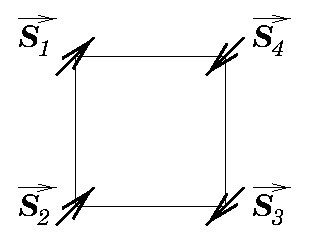
\includegraphics[clip,height=30mm,width=40mm]{1997phy3-2.eps}
%\includegraphics[clip]{1997phy3-2.eps hscale=0.6 vscale=0.6}
\end{center}
}
\SubQuestion
上の4個のスピン系の低温での磁化率の漸近形、高温での磁化率の漸近形はどうなるか。理由をつけて答えよ。

\end{subquestions}
\end{question}
\begin{answer}{専攻 問題3}{}
% ↑↓の定義
\newcommand{\Up}{\uparrow}
\newcommand{\Down}{\downarrow}

\begin{subanswers}
\SubAnswer

\parbox[t]{60mm}{
$\vec{S_1}+\vec{S_2}=\vec{S}$とおく。このとき、ハミルトニアンは、
\[ {\cal{H}}=\frac{1}{2}J (\vec{S}^2-\vec{S_1}^2-\vec{S_2}^2) \]
と表わせられる。各運動量の一般論から、右表のように表すことができる。}
\parbox[t]{100mm}{\vspace*{-5mm}
\quad 
\begin{center}
\begin{tabular}{|c|c|c|} \hline
固有状態        & $\vec{S}^2$の固有値 & $\cal{H}$の固有値  \\ \hline\hline
$| \Up_1,\Up_2 >$     &                   &                  \\
$\frac{1}{\sqrt{2}}(|\Up_1,\Down_2>+|\Down_1,\Up_2>)$  &     $2$             & $\frac{1}{4}J$     \\
$|\Down_1,\Down_2>$  &                   &                  \\ \hline
$\frac{1}{\sqrt{2}}(|\Up_1,\Down_2>-|\Down_1,\Up_2>)$  &     0             & $-\frac{3}{4}J$    \\ \hline
\end{tabular}
\end{center}}

但し、$\Up,\Down$は、$\vec{S_i^z}\quad (i=1,2)$の固有値が$\frac{1}{2}$または、$-\frac{1}{2}$の状態を表し、全体として直積を表すものとする。
\SubAnswer
\parbox[t]{65mm}{
それぞれの固有値を固有状態を表にしてまとめると、右表のようになる。

よって、分配関数$Z$は、
\[\hspace{-15mm} Z = {\rm{Tr}}[\exp(-\beta{\cal{H}})]  \]
\[\hspace{-15mm}   =  {\exp}(-\frac{1}{4}J\beta)(1+2{\cosh}( g \mu_BH\beta)+\exp(J\beta))\]
}
\parbox[t]{95mm}{\vspace*{-5mm}
\begin{center}
\begin{tabular}{|c|c|c|c|} \hline
固有状態 & $\vec{S}^2$ & $S^z$ & $\cal{H}$の固有値 \\ \hline\hline
$|\Up_1,\Up_2>$ &   2   &   1 & $-g\mu_B H+\frac{1}{4} J $ \\ \hline
$\frac{1}{\sqrt{2}}(|\Up_1,\Down_2>+|\Down_1,\Up_2>)$ & 2 & 0 & $\frac{1}{4} J$ \\ \hline
$|\Down_1,\Down_2>$ & 2 & -1 & $g\mu_B H+\frac{1}{4} J $ \\ \hline
$\frac{1}{\sqrt{2}}(|\Up_1,\Down_2>-|\Down_1,\Up_2>)$ & 0 & 0 & $-\frac{3}{4} J$ \\ \hline
\end{tabular}
\end{center}
}

\SubAnswer
\[ M=\frac{1}{\beta}\Partial{\ln Z}{H}=g\mu_B \frac{2\sinh(g\mu_B H \beta)}{1+2\cosh(g\mu_B H \beta)+\exp(J\beta)} \]
$\sinh(x)=x+{\rm{O}}(x^3)$\quad ,\quad $\cosh(x)=1+{\rm{O}}(x^2)$を用いて、
\[ \frac{M}{H}=g\mu_B \frac{2(g\mu_B H \beta)+{\rm{O}}(H^3)}{H(3+\exp(-J\beta)+{\rm{O}}(H^2))}= \frac{2 (g\mu_B)^2 \beta }{3+\exp(J\beta)}(1+{\rm{O}}(H^2)) \]
よって、
\[ \lim_{H\rightarrow 0} \frac{M}{H}= \frac{2(g\mu_B)^2 \beta }{3+\exp(J\beta)} \]
\parbox[t]{90mm}{(i)$k_B T \gg J$ ($\beta J \ll 1$)のとき
\[\hspace{-5mm} \chi=\frac{2(g\mu_B)^2 \beta}{4+{\rm{O}}(J\beta)}= \frac{(g\mu_B)^2}{2}\beta (1+{\rm{O}}(J\beta)) \sim \frac{(g\mu_B)^2}{2}\beta \]

(ii)$k_B T \ll J $($\beta J \gg 1$)のとき
\[\hspace{-5mm} \chi = \frac{2\beta(g\mu_B)^2}{\exp(J\beta)}(1+\frac{1}{3}\exp(-J\beta)) \sim \frac{2(g\mu_B)^2 \beta}{\exp(J\beta)} \]

この結果を図示すると右図のようになる。
}\parbox[t]{70mm}{\vspace*{-7mm}
\begin{center}
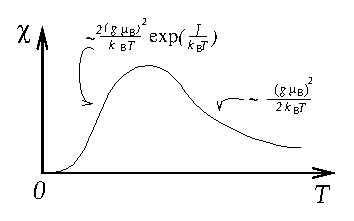
\includegraphics[clip,height=40mm,width=55mm]{1997phy3-3.eps}
\end{center}
}

\SubAnswer
$\vec{S}=\vec{S_\alpha}+\vec{S_\beta}$とし、$\vec{S_\alpha}=\vec{S_1}+\vec{S_3}$\quad ,\quad $\vec{S_\beta}=\vec{S_2}+\vec{S_4}$とすると、
\[ {\cal{H}}=\frac{1}{2}J (\vec{S_{ }}^2 -\vec{S_\alpha}^2-\vec{S_\beta}^2 ) \]
$\vec{S\alpha}$,$\vec{S_\beta}$の固有値は{\bf{1}}で行った通りなので、この2つを合成することを考えれば良い。書き漏れがないことを確かめるためにも、全体の次元が16存在していることを確かめることは有用である。

\parbox[t]{50mm}{
(i)$S_\alpha=1$,$S_\beta=1$のとき

\begin{tabular}{|c|c|c|}\hline
$S$ & $\cal{H}$の固有値 & 次元 \\ \hline\hline
$2$ & $J$                 & $ 5 $ \\ \hline
$1$ & $-J$                & $ 3 $ \\ \hline
$0$ & $-2J$               & $ 1 $ \\ \hline
\end{tabular}}
\parbox[t]{50mm}{
(ii)$S_\alpha=1,S_\beta=0$あるいは、\\
$S_\alpha=0,S_\beta=1$のとき

\begin{tabular}{|c|c|c|}\hline
$S$ & $\cal{H}$の固有値 & 次元 \\ \hline \hline 
$1$ & $0$                 & $ 3 $ \\ \hline
\end{tabular}

(つまり、全部で次元は$6$)
}
\parbox[t]{50mm}{
(iii)$S_\alpha=0,S_\beta=0$のとき 

\begin{tabular}{|c|c|c|}\hline
$S$ & $\cal{H}$の固有値 & 次元 \\ \hline \hline
$0$ & $0$              & $ 1 $ \\ \hline
\end{tabular} }

\SubAnswer
高温では、各々のスピンの振る舞いのランダム性が増加する。つまり、$J(\vec{S_1}+\vec{S_3})\cdot (\vec{S_2}+\vec{S_4})$による個々のスピン間の相互作用の効果が小さくなり、スピン個々がもっている性質に依存する。よって、$\chi$はスピンの個数に比例する。(エネルギー差による存在比(population)に差が見られなくなる。)つまり、スピン$n$個のときの磁化率を$\chi_n$とすれば、
\[ \frac{\chi_2}{2} \sim \frac{\chi_4}{4} \sim \frac{\chi_n}{n} \]
よって、
\[ \chi_4 \sim 2 \chi_2 = (g\mu_B)^2 \beta \]
となる。

低温において、ほとんどが基底状態になる。2スピン系との共通点として、(但し、基底状態と第一励起状態の波動関数を$|\Psi_0>,|\Psi_{1(i)}>$(添字$i$は、縮重を考慮している。)とし、磁気モーメントを表す演算子を$\Operator{M}(=g\mu_B S_z)$とする。)
\begin{itemize}
\item 基底状態において、${\displaystyle{\Mean{M_0}=<\Psi_0| \Operator{M} | \Psi_0>=0}}$である。
\item 第一励起状態において ${\displaystyle{\Mean{M_i}=<\Psi_{1(i)}|\Operator{M} | \Psi_{1(i)}> \neq 0}}$\quad , \quad ${\displaystyle{\sum_{i}\Mean{M_i}= \sum_{i}<\Psi_{1(i)}|\Operator{M} | \Psi_{1(i)}> =0}}$である。
\end{itemize}
{\bf{3}}の解答を見ると、分母が基底状態から励起状態への励起率を表し、分子が磁場を掛けたときの第一励起状態の応答を表している。同一エネルギー準位(第一励起状態)についての応答を考えるので、そのときの$M$は、
\[ M=\frac{\sum_i M_i \exp\{-\beta(E^{(0)}-M_i H)\}}{\sum_j \exp\{-\beta (E^{(0)}-M_j H)\}} \hspace{10mm} \Yueni \Deriver{}{H} M|_{H=0,\beta>>1}\simeq \sum_i M_i^2 \beta \]
となる。ただし、$E^{(0)}$は$H$に因らない摂動($H$をかける)以前のエネルギーを示している。よって、第一励起状態と基底状態のエネルギー差を$\Delta E (= <\Psi_{1(i)}|{\cal{H}}|\Psi_{1(i)}>-<\Psi_0|{\cal{H}}|\Psi_0>)$として、

\[ \chi \sim \frac{\sum_i M_i^2}{\exp((\Delta E) \beta)} \beta \]
となることが分かる。よって、
\[ \chi_4 \sim \frac{2(g\mu_B)^2}{\exp(J \beta)} \beta \]
となる。ちなみに、地道に計算すると、
\begin{equation}
\chi =\frac{(g\mu_B)^2 (10 \exp(-J\beta)+2\exp(J\beta)+4) \beta }{5\exp(-J\beta)+3\exp(J\beta)+\exp(2J\beta)+7} \sim \left\{\begin{array}{ccc}
(g \mu_B)^2 \beta & \hspace{5mm} & \beta \rightarrow 0 \\
\frac{2(g \mu_B)^2 \beta}{\exp(J\beta)} & & \beta \rightarrow \infty
\end{array}\right. \eqname{zimichi}   
\end{equation}
となる。各自、確かめてほしい。(次元が16あることに注意)また、『低温のときは、基底状態と励起状態のみで計算しても低温極限では、磁化率は同じ解になり、高温極限では、$\beta J=0$の仮定のもとで計算しても同じ解が得られる。』ことから、磁化率の振る舞いを論じても良い。 

{\bf{[補足1]}} $\chi$に対する一般解を求めてみよう。磁場を摂動的に考えて、
\[ E_n=E_n^{(0)}-M_n H  \hspace{10mm}(但し、E_n^{(0)}はHに因らない摂動以前のエネルギーを示す。)\]
磁化$M$は$M=\ds\frac{\sum_n M_n \exp(-\beta E_n)}{\sum_m \exp(-\beta E_m)}$で与えられる。さらに、$M|_{H=0}=0$を仮定する。この仮定は、自発磁化が存在しない場合にのみ、許される。(この問題に対して適切である。) 磁化率$\chi$は、
\begin{equation}
\lim_{H\rightarrow 0}\frac{M}{H}\simeq \Deriver{}{H} M|_{H=0}=\frac{\sum_n M_n^2 \exp(-\beta E_n)}{\sum_m \exp(-\beta E_m)}\beta  \eqname{hosoku2-1}
\end{equation}

これに対し、スピンの合成の結果({\bf{[補足2]}}参照)の値を代入すると、地道に計算した結果の$\chi$(\eqhref{zimichi})が得られる。

 ここで、\eqhref{hosoku2-1}の式で得られた$\chi$の低温極限と高温極限について調べてみよう。低温極限については、式の形から、解答に示した物理的考察によって得られた低温極限の近似式が正しいことは明らかである。高温極限については、
\[ \Deriver{^2}{\beta^2}(e^{\beta}+e^{-\beta})^n =n(n-1)(e^\beta+e^{-\beta})^{n-2}(e^\beta-e^{-\beta})^2+n(e^\beta+e^{-\beta})^n \]
両辺に$\beta=0$を代入し、左辺を展開することにより、二項係数$_i{\rm C}_j$を用いて、
\[ _n{\rm C}_0 n^2+_n{\rm C}_1(n-2)^2+_n{\rm C}_2 (n-4)^2 \cdots +_n{\rm C}_n(-n)^2 = 2^n\times n \]
これを用いて、高温極限の近似式は、$M_n$がスピンの合成より得られたことを考えると、全スピンの数$N$(この問題では$N=4$)として、
\[ \frac{\sum_n M_n^2 \exp(-\beta E_n)}{\sum_m \exp(-\beta E_m)}\beta \sim \frac{\frac{(g\mu_B)^2}{4}N 2^N}{2^N} \beta =\frac{N(g\mu_B)^2}{4}\beta \propto N \]
となるから、解答に示した物理的考察によって得られた高温極限の近似式が正しいことが示せたことになる。

{\bf{[補足2]}} 問題{\bf{4}}で、地道に計算すると、スピン4つの合成を行わねばならない。最初にスピン二つずつを合成し、最後にもう一度合成した方が分かりやすいだろう。スピンの合成は、単に計算していけばよいので、計算結果のみ示すこととする。(下の(i),(ii),(iii)の場合わけは、問題{\bf{4}}の振り方と同じである。)

 (i)$S_\alpha=1$,$S_\beta=1$のとき

(イ)$S=2$($S_z=\ds\frac{M}{g\mu_B}$)

\begin{tabular}{|c|c|}\hline
$S_z$ & スピン波動関数 \\ \hline \hline
$2$ & $|\Up,\Up,\Up,\Up>$ \\ \hline
$1$ & $\frac{1}{2}\{ |\Down,\Up,\Up,\Up>+|\Up,\Down,\Up,\Up>+|\Up,\Up,\Down,\Up>+|\Up,\Up,\Up,\Down>\}$ \\ \hline
$0$ & $\frac{1}{\sqrt{6}}\{|\Down,\Down,\Up,\Up>+|\Down,\Up,\Down,\Up>+|\Down,\Up,\Up,\Down>+|\Up,\Down,\Down,\Up>+|\Up,\Down,\Up,\Down>+|\Up,\Up,\Down,\Down>\}$ \\ \hline
$-1$ & $\frac{1}{2}\{ |\Up,\Down,\Down,\Down>+|\Down,\Up,\Down,\Down>+|\Down,\Down,\Up,\Down>+|\Down,\Down,\Down,\Up>\}$ \\ \hline
$-2$ & $|\Down,\Down,\Down,\Down>$ \\ \hline
\end{tabular}

(ロ)$S=1$

\begin{tabular}{|c|c|}\hline
$S_z$ & スピン波動関数 \\ \hline \hline
$1$ & $\frac{1}{2}\{|\Up,\Up,\Up,\Down>+|\Up,\Up,\Down,\Up>-|\Up,\Down,\Up,\Up>-|\Down,\Up,\Up,\Up>\}$ \\ \hline
$0$ & $\frac{1}{\sqrt{2}}\{ |\Up,\Up,\Down,\Down>-|\Down,\Down,\Up,\Up> \}$ \\ \hline
$-1$ & $\frac{1}{2}\{|\Up,\Down,\Down,\Down>+|\Down,\Up,\Down,\Down>-|\Down,\Down,\Down,\Up>-|\Down,\Down,\Up,\Down>\}$ \\ \hline
\end{tabular}

(ハ)$S=0$

\begin{tabular}{|c|c|}\hline
$S_z$ & スピン波動関数 \\ \hline \hline
$0$ & $\frac{1}{2\sqrt{2}}\{ 
2|\Up,\Up,\Down,\Down>+2|\Down,\Down,\Up,\Up>-|\Up,\Down,\Up,\Down>-|\Up,\Down,\Down,\Up>-|\Down,\Up,\Up,\Down>-|\Down,\Up,\Down,\Up>
\}$ \\ \hline
\end{tabular}

(ii) (a)$S_\alpha=1,S_\beta=0$のとき

\begin{tabular}{|c|c|}\hline
$S_z$ & スピン波動関数 \\ \hline \hline
$1$ & $\frac{1}{\sqrt{2}}\{ |\Up,\Up,\Up,\Down>-|\Up,\Up,\Down,\Up>\}$ \\ \hline
$0$ & $\frac{1}{2}\{|\Down,\Up,\Up,\Down>+|\Up,\Down,\Up,\Down>-|\Down,\Up,\Down,\Up> -|\Up,\Down,\Down,\Up>\}$ \\ \hline
$-1$ & $\frac{1}{\sqrt{2}}\{ |\Down,\Down,\Up,\Down>-|\Down,\Down,\Down,\Up>\}$ \\ \hline
\end{tabular}

%%%%
(b)$S_\alpha=0,S_\beta=1$のとき

\begin{tabular}{|c|c|}\hline
$S_z$ & スピン波動関数 \\ \hline \hline
$1$ & $\frac{1}{\sqrt{2}}\{ |\Up,\Down,\Up,\Up>-|\Down,\Up,\Up,\Up>\}$ \\ \hline
$0$ & $\frac{1}{2}\{|\Up,\Down,\Down,\Up>+|\Up,\Down,\Up,\Down>-|\Down,\Up,\Down,\Up> -|\Down,\Up,\Up,\Down>\}$ \\ \hline
$-1$ & $\frac{1}{\sqrt{2}}\{ |\Up,\Down,\Down,\Down>-|\Down,\Up,\Down,\Down>\}$ \\ \hline
\end{tabular}

(iii)$S_\alpha=0,S_\beta=0$のとき

\begin{tabular}{|c|c|}\hline
$S_z$ & スピン波動関数 \\ \hline \hline
$0$ & $\frac{1}{2}\{
|\Up,\Down,\Up,\Down>+|\Down,\Up,\Down,\Up>-|\Up,\Down,\Down,\Up>-|\Down,\Up,\Up,\Down> \}$ \\ \hline
\end{tabular}

\end{subanswers}
\end{answer}

\end{document}





